\documentclass[12pt,a4paper]{article}
\usepackage[utf8]{inputenc}
%\usepackage[left=2.00cm,right=2.00cm,top=2.00cm,bottom=2.00cm]{geometry}
\usepackage{transparent}
\usepackage{amsmath}                                 % AMS Math Package
\usepackage[utf8]{inputenc}
\usepackage{amsthm}                                  % Theorem Formatting
\usepackage{amssymb}                                 % Math symbols such as \mathbb
\usepackage{graphicx}                                % Allows for eps images
\usepackage[dvips,a4paper,margin=1in,bottom=1in]{geometry}
\usepackage{tensor}

\usepackage{titlesec}
\usepackage{csquotes}

\titlespacing\section{0pt}{12pt plus 4pt minus 2pt}{0pt plus 2pt minus 2pt}
\titlespacing\subsection{0pt}{12pt plus 4pt minus 2pt}{0pt plus 2pt minus 2pt}
\titlespacing\subsubsection{0pt}{12pt plus 4pt minus 2pt}{0pt plus 2pt minus 2pt}

% Sets margins and page size

\usepackage{amsmath, esint,mathrsfs}
\def\doubleunderline#1{\underline{\underline{#1}}}
\renewcommand{\labelenumi}{(\alph{enumi})}                % Use letters for enumerate

\usepackage{enumerate}
\usepackage{caption}
\usepackage[]{algorithm2e}

\usepackage{listings}
\usepackage{xcolor}

\definecolor{codegreen}{rgb}{0,0.6,0}
\definecolor{codegray}{rgb}{0.5,0.5,0.5}
\definecolor{codepurple}{rgb}{0.58,0,0.82}
\definecolor{backcolour}{rgb}{0.95,0.95,0.92}

\lstdefinestyle{mystyle}{
	language=Python,
	backgroundcolor=\color{backcolour},   
	commentstyle=\color{codegreen},
	keywordstyle=\color{magenta},
	numberstyle=\tiny\color{codegray},
	stringstyle=\color{codepurple},
	basicstyle=\ttfamily\footnotesize,
	breakatwhitespace=false,         
	breaklines=true,                 
	captionpos=b,                    
	keepspaces=true,                 
	numbers=left,                    
	numbersep=5pt,                  
	showspaces=false,                
	showstringspaces=false,
	showtabs=false,                  
	tabsize=2
}

\lstset{style=mystyle}

\newcommand{\gv}[1]{\ensuremath{\mbox{\boldmath$ #1 $}}} 
\newcommand{\uv}[1]{\ensuremath{\mathbf{\hat{#1}}}}       % enhetsvektor
\newcommand{\abs}[1]{\left| #1 \right|}                   % abslouttverdi
\newcommand{\avg}[1]{\left< #1 \right>}                   % gjennomsnitt

\newcommand{\der}[2]{\frac{\text{d} #1}{\text{d} #2}}     % derivert
\newcommand{\dd}[2]{\frac{\text{d}^2 #1}{\text{d}#2^2}}   % dobbelderivert
\newcommand{\pd}[2]{\frac{\partial #1}{\partial #2}}      % partiellderiverte
\newcommand{\pdd}[2]{\frac{\partial^2 #1}{\partial #2^2}} % doble partiellderiverte

% Kvantemekanikk:

\newcommand{\ket}[1]{\left| #1 \right>}                    % for Dirac kets
\newcommand{\bra}[1]{\left< #1 \right|}                    % for Dirac bras
\newcommand{\braket}[2]{\left< #1 \vphantom{#2} \right|
	\left. #2 \vphantom{#1} \right>}                       % for Dirac brackets
\newcommand{\matrixel}[3]{\left< #1 \vphantom{#2#3} \right|
	#2 \left| #3 \vphantom{#1#2} \right>}                  % for Dirac matrix elements

% Vektoranalyse

\newcommand{\grad}[1]{\gv{\nabla} #1}                      % gradient
\let\divsymb=\div                                          % nytt navn til div
\renewcommand{\div}[1]{\gv{\nabla} \cdot \v{#1}}           % divergens
\newcommand{\curl}[1]{\gv{\nabla} \times \v{#1}}           % curl


% div macros

\newcommand{\iu}{\textup{i}} % imaginary unit
\newcommand{\e}{\textup{e}} % exponent
\newcommand{\intd}[1]{\int\text{d}#1}

% document layout

\setlength{\parindent}{0em}
\setlength{\parskip}{1em}
\setlength{\parindent}{0pt}

\usepackage{fancyhdr}
\usepackage{titlesec}

\usepackage{nameref}

\author{Sondre Duna Lundemo}

\newcommand\bluetextit[1]{\textcolor{blue}{\textit{\sffamily#1}}}
\newcommand\bluetextbf[1]{\textcolor{blue}{\textbf{\sffamily#1}}}

\pagestyle{fancy}
\renewcommand{\headrulewidth}{0.5pt}
\fancyhf{}
\rhead{\textit{\fontfamily{cmr}\selectfont Sondre Duna Lundemo}}
\lhead{\small \textsc{\rightmark}}
\cfoot{\textemdash \, \thepage \, \textemdash}

\titleformat*{\section}{\bfseries \Large}
\titleformat*{\subsection}{\bfseries\large}
\titleformat*{\subsubsection}{\bfseries \normalsize}

\fancypagestyle{titlepage}{
	\fancyhf{}
	\fancyfoot[C]{$\dagger$\href{mailto:sondre@duna.no}{\texttt{sondre@duna.no}}}
	\fancyfootoffset{-4cm}
	\renewcommand{\headrulewidth}{0pt}
	\renewcommand\footrulewidth{0.5pt}
}

% theoremstyles

\theoremstyle{plain}
\newtheorem{thm}{Theorem}
\newtheorem{axiom}{Axiom}

\theoremstyle{definition}

\newtheorem{definition}{Definition}
\newtheorem{lemma}{Lemma}
\newtheorem{cor}{Corollary}
\newtheorem{prop}{Proposition}

\theoremstyle{remark}

\newtheorem{remark}{Remark}
\newtheorem{notation}{Notation}

\usepackage{enumitem}

\def\be{\begin{equation}}
\def\ee{\end{equation}}

\def\bse{\begin{equation*}}
\def\ese{\end{equation*}}

\def\bt{\begin{thm}}
\def\et{\end{thm}}

\def\bl{\begin{lemma}}
\def\el{\end{lemma}}

\def\bc{\begin{cor}}
\def\ec{\end{cor}}

\def\br{\begin{remark}}
\def\er{\end{remark}}

\def\bal{\begin{align}}
	\def\eal{\end{align}}
	
\def\bd{\begin{definition}}
	\def\ed{\end{definition}}

\def\bit{\begin{itemize}}
	\def\eit{\end{itemize}}

\def\bt{\begin{thm}}
	\def\et{\end{thm}}

\let\vaccent=\v % rename builtin command \v{} to \vaccent{}
\renewcommand{\v}[1]{\ensuremath{\mathbf{#1}}} % vektor

%miscellaneous shortcuts

\providecommand{\AA}{\mathbb{A}}
\providecommand{\BB}{\mathbb{B}}
\providecommand{\CC}{\mathbb{C}}
\providecommand{\DD}{\mathbb{D}}
\providecommand{\EE}{\mathbb{E}}
\providecommand{\FF}{\mathbb{F}}
\providecommand{\GG}{\mathbb{G}}
\providecommand{\HH}{\mathbb{H}}
\providecommand{\II}{\mathbb{I}}
\providecommand{\JJ}{\mathbb{J}}
\providecommand{\KK}{\mathbb{K}}
\providecommand{\LL}{\mathbb{L}}
\providecommand{\MM}{\mathbb{M}}
\providecommand{\NN}{\mathbb{N}}
\providecommand{\OO}{\mathbb{O}}
\providecommand{\PP}{\mathbb{P}}
\providecommand{\QQ}{\mathbb{Q}}
\providecommand{\RR}{\mathbb{R}}
\providecommand{\SS}{\mathbb{S}}
\providecommand{\TT}{\mathbb{T}}
\providecommand{\UU}{\mathbb{U}}
\providecommand{\VV}{\mathbb{V}}
\providecommand{\WW}{\mathbb{W}}
\providecommand{\XX}{\mathbb{X}}
\providecommand{\YY}{\mathbb{Y}}
\providecommand{\ZZ}{\mathbb{Z}}

\providecommand{\A}{\mathcal{A}}
\providecommand{\B}{\mathcal{B}}
\providecommand{\C}{\mathcal{C}}
\providecommand{\D}{\mathcal{D}}
\providecommand{\E}{\mathcal{E}}
\providecommand{\F}{\mathcal{F}}
\providecommand{\G}{\mathcal{G}}
\providecommand{\H}{\mathcal{H}}
\providecommand{\I}{\mathcal{I}}
\providecommand{\J}{\mathcal{J}}
\providecommand{\K}{\mathcal{K}}
\providecommand{\L}{\mathcal{L}}
\providecommand{\M}{\mathcal{M}}
\providecommand{\N}{\mathcal{N}}
\providecommand{\CO}{\mathcal{O}}
\providecommand{\P}{\mathcal{P}}
\providecommand{\Q}{\mathcal{Q}}
\providecommand{\R}{\mathcal{R}}
\providecommand{\S}{\mathcal{S}}
\providecommand{\T}{\mathcal{T}}
\providecommand{\U}{\mathcal{U}}
\providecommand{\V}{\mathcal{V}}
\providecommand{\W}{\mathcal{W}}
\providecommand{\X}{\mathcal{X}}
\providecommand{\Y}{\mathcal{Y}}
\providecommand{\Z}{\mathcal{Z}}

\usepackage{hyperref}
\hypersetup{colorlinks=true,linkcolor=blue}

\begin{document}
	
\begin{titlepage}
	\begin{center}
	\setlength{\parskip}{0em}
	\thispagestyle{titlepage}
	
	\centering{
		\Huge{\textbf{ Numerical simulation of magnons }}
	}

	\vspace{4mm}
	
	\large{\textbf{Sondre Duna Lundemo}}$\dagger$
	
	\normalsize{Department of Physics, Norwegian University of Science and Technology, Trondheim Norway \\
	TFY4235 - Computational physics
	}

	(\textit{Last updated on \today})
	\end{center}

	\setlength{\parindent}{2em}
	
		We simulate a linear chain of spins through numerically solving the Landau-Lifschitz-Gilbert equation with Heun's method. The simple case of a single spin is compared to an analytical solution, and the more complicated systems are compared to known results in spin wave theory. Magnetic waves (magnons) propagating on the chain are demonstrated to emerge from this equation and their behaviour for different parameter values are discussed.
	
	\begin{figure}
		
	\end{figure}
	

\end{titlepage}

\newpage
\setlength{\parskip}{0em}
\tableofcontents
\setlength{\parskip}{1em}
\newpage

\part{Introduction}

\section{Theoretical background}

The hamiltonian governing the dynamics of a chain of spins is
\begin{equation}\label{eq:hamiltionian}
	H = - \frac{1}{2} \sum_{j,k}^{N} J_{jk} \mathbf{S}_j \cdot \mathbf{S}_k - d_z \sum_{j=1}^{N} (S_{j,z})^2 - \mu \sum_{j=1}^{N} \mathbf{B}_j \cdot \mathbf{S}_j,
\end{equation}

And the time-dependence is governed by the Landau-Lifshitz-Gilbert equation (LLG) 
\begin{equation}\label{eq:llg}
	\der{\mathbf{S}_j}{t} = \frac{-\gamma}{\mu(1 + \alpha^2)} \left[ \mathbf{S}_j \times \mathbf{H}_j + \alpha \mathbf{S}_j \times (\mathbf{S}_j \times \mathbf{H}_j) \right]
\end{equation}
where
\begin{equation}\label{eq:ef_field}
	\mathbf{H}_j = -\pd{H}{\mathbf{S}_j} + \boldsymbol{\xi}_j.
\end{equation}

In the absence of noise, $\boldsymbol{\xi}_j \equiv 0$, we can find an explicit relation for the effective field $\mathbf{H}_j$ in \eqref{eq:ef_field}. This can be done by noting that 
\begin{align*}
	-\pd{H}{\mathbf{S}_j} &= \frac{1}{2}\sum_{i,k}^{N} J_{ik} \frac{\partial}{\partial \mathbf{S}_j} \left( \mathbf{S}_i \cdot \mathbf{S}_k \right) + d_z \sum_{i=1}^{N} \frac{\partial }{\partial \mathbf{S}_j}(\mathbf{S}_i \cdot \mathbf{e}_z)^2 + \mu \sum_{i=1}^{N} \frac{\partial }{\partial \mathbf{S}_j} \mathbf{B}_i \cdot \mathbf{S}_i \\
	&= \frac{1}{2}\sum_{i,k}^{N} J_{ik} \left( \delta_{ij} \mathbf{S}_k + \delta_{jk} \mathbf{S}_i \right) + d_z \sum_{i=1}^N 2 \delta_{ij} (\mathbf{S}_i \cdot \mathbf{e}_z) \mathbf{e}_z + \mu \sum_{i=1}^N \mathbf{B}_i \delta_{ij} \\
	&= \sum_{i=1}^N J_{ij} \mathbf{S}_i + 2d_z S_{j,z} \mathbf{e}_z + \mu \mathbf{B} \\
	&= \sum_{i \in \mathcal{N}_j} J_{ij} \mathbf{S}_i + 2d_z S_{j,z} \mathbf{e}_z + \mu \mathbf{B}, 
\end{align*}

where we in the last transition have made further simplifications by only performing the sum over the nearest neighbours $\mathcal{N}_j$ of $j$. Using this expression we may rewrite the LLG in \eqref{eq:llg} as
\begin{align}\label{eq:llg_simplified}
	\der{\mathbf{S}_j}{t} = \frac{-\gamma}{\mu(1 + \alpha^2)} \Bigg[ \mathbf{S}_j &\times \left( \sum_{i \in \mathcal{N}_j} J_{ij} \mathbf{S}_i + 2d_z S_{j,z} \mathbf{e}_z + \mu \mathbf{B} \right) \nonumber \\
	+ \alpha \mathbf{S}_j \times \Bigg[  \mathbf{S}_j  &\times \left( \sum_{i \in \mathcal{N}_j} J_{ij} \mathbf{S}_i + 2d_z S_{j,z} \mathbf{e}_z + \mu \mathbf{B} \right) \Bigg] \Bigg]. 
\end{align}
It is the form of the LLG in equation \ref{eq:llg_simplified} that we will use in the implementation.
\newpage

\part{Code overview}

\section{General structure}

\section{Remarks on performance}
\newpage

\part{Results and discussion}
\section{Single spin}
\subsection{Precession of spin in uniform magnetic field}

We simulate the time evolution of a single spin $\mathbf{S}$ in the presence of a uniform magnetic field $\mathbf{B} = (0,0,B_0)^T$ in the $\mathbf{e}_z$-direction. The components of the spin at equidistant time steps during one period are shown in figure \ref{fig:spin_1}. As expected, we see that the spin precesses around the effective field $\mathbf{H}$, which in this case is given by
\[
	\mathbf{H} = -\pd{H}{\mathbf{S}} = \frac{\partial}{\partial \mathbf{S}}\left( \mu \mathbf{B} \cdot \mathbf{S} \right) =\mu \mathbf{B},
\]
in the absence of damping and anisotropy.

\begin{figure}[htb]
	\centering
	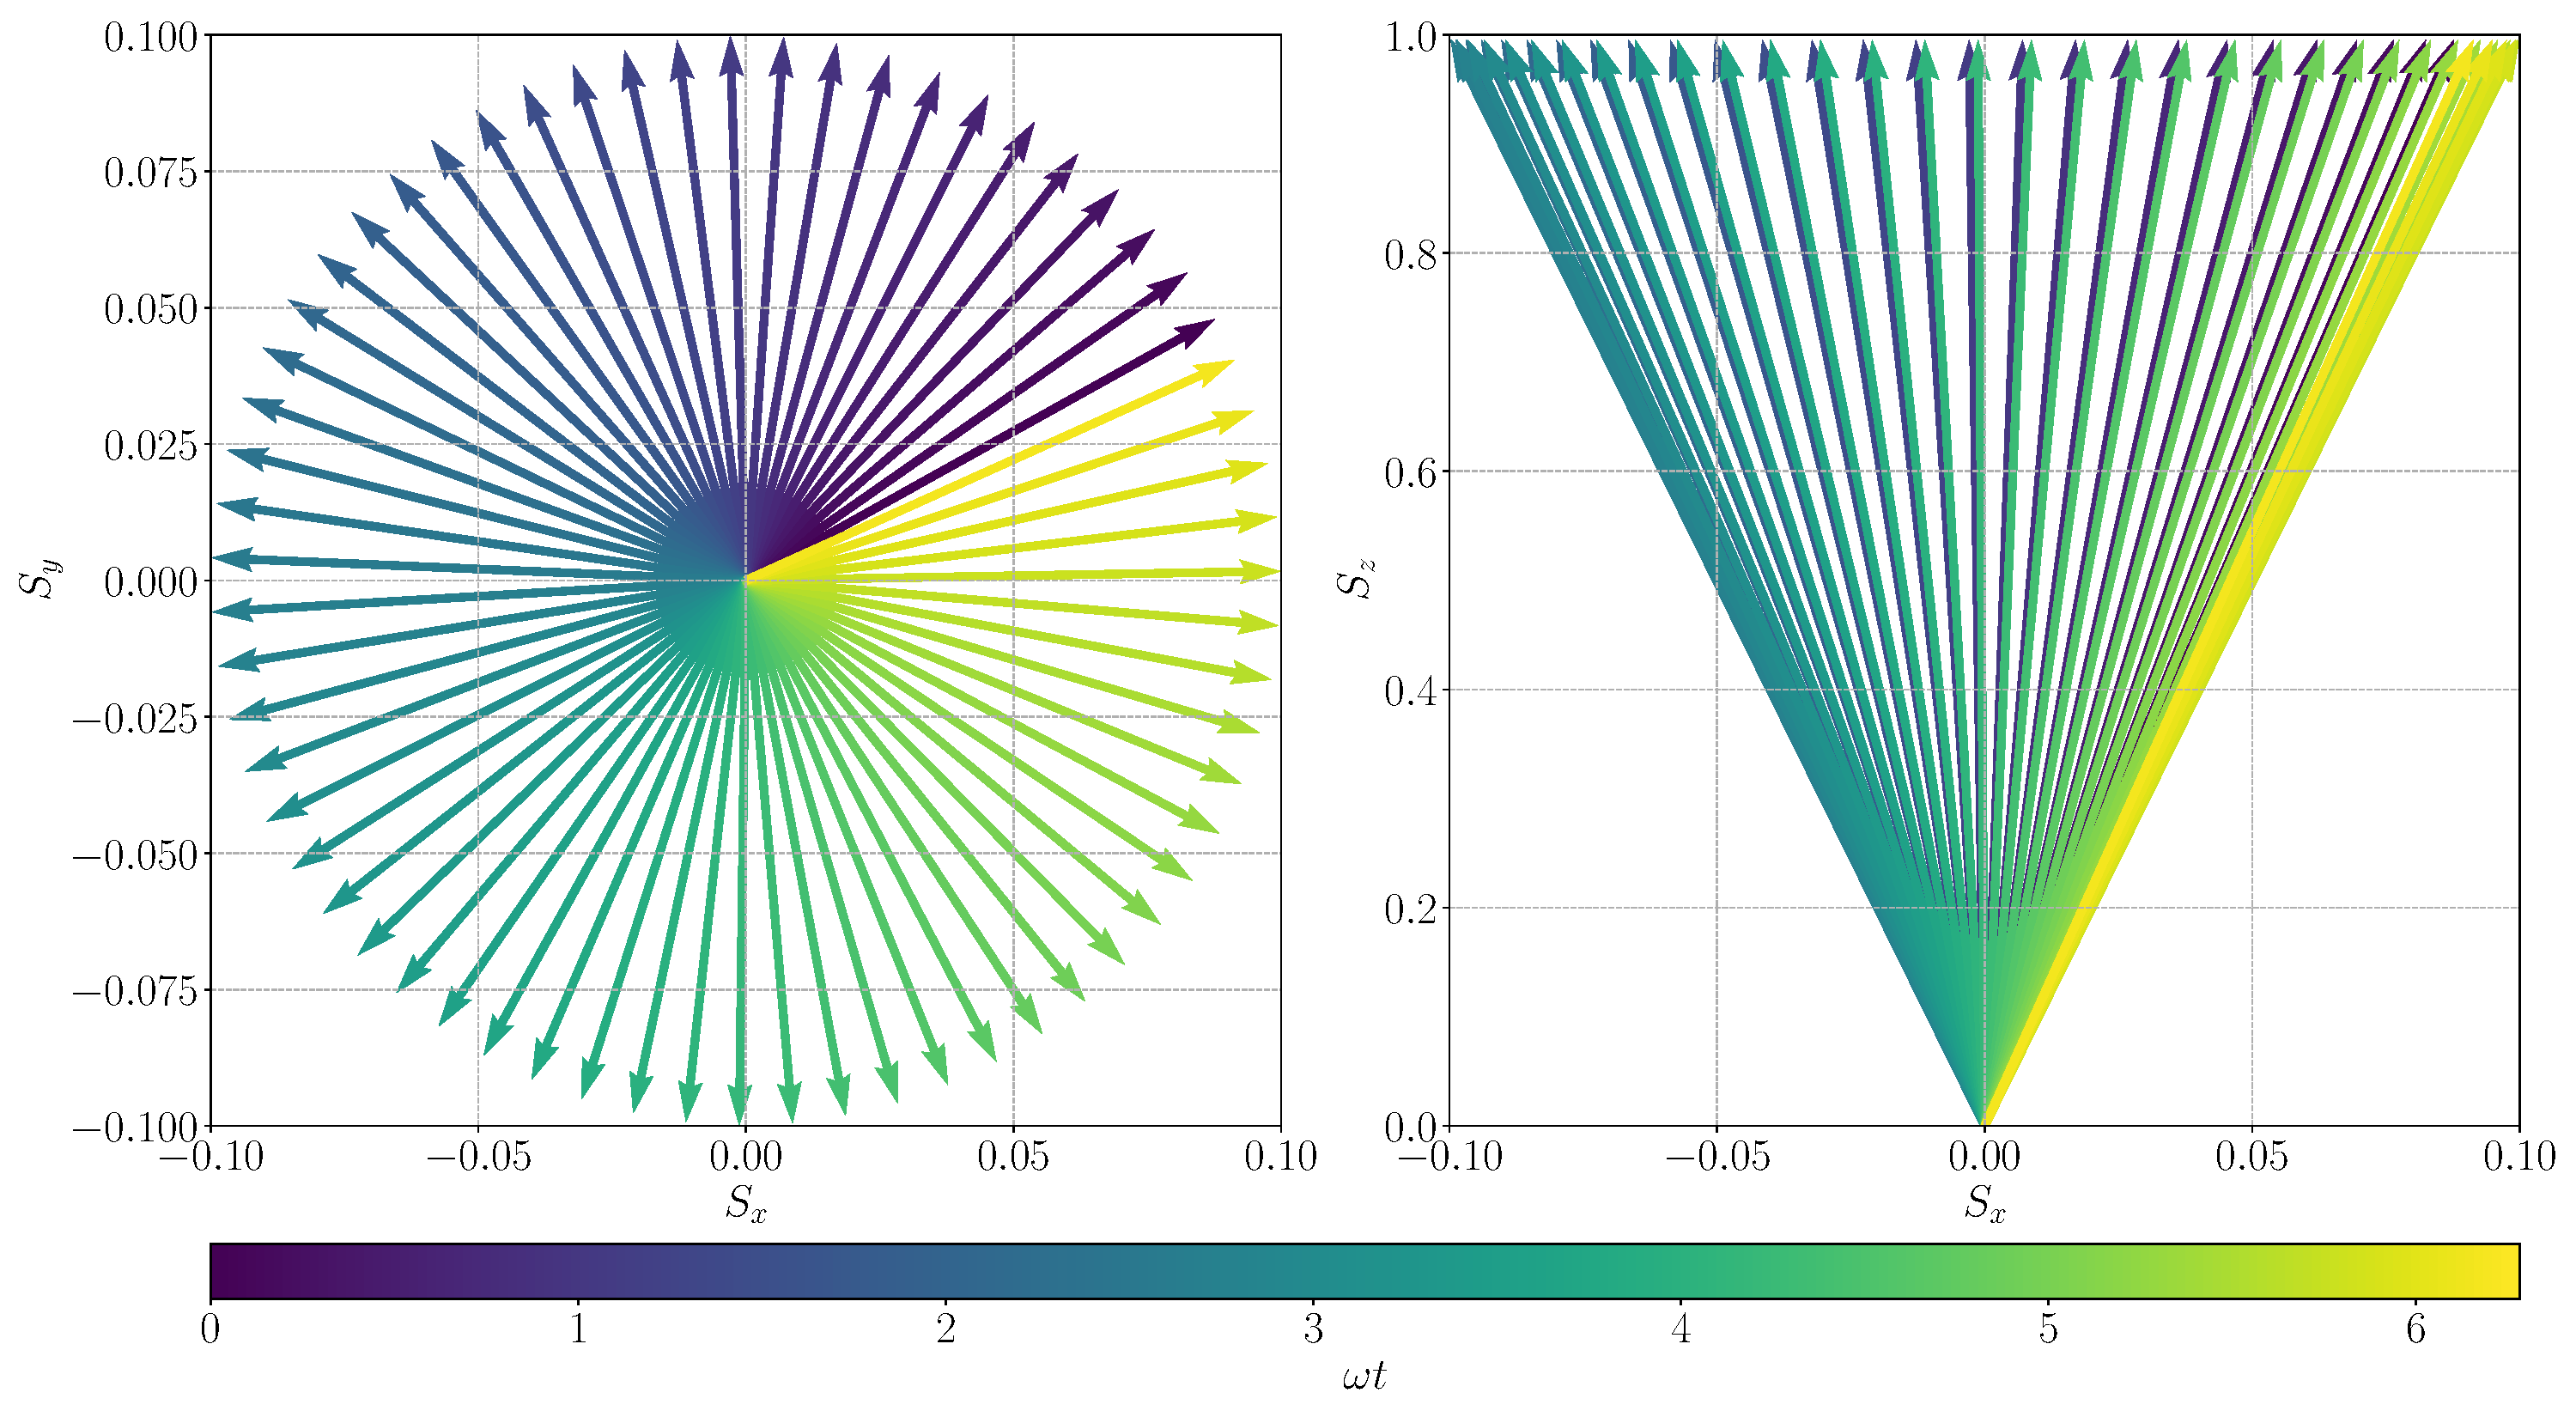
\includegraphics[width=\columnwidth]{../fig/magnet_xy_1}
	\caption{The figure shows the $x$ and $y$ component of the spin during one period in a uniform magnetic field without further interactions.}
	\label{fig:spin_1}
\end{figure}

In this particular case, we can easily find an analytical solution to compare with. The LLG-equation reads
\[
	\partial_t \mathbf{S} = -\frac{\gamma}{\mu} \mathbf{S} \times \mathbf{B}.
\]
As $\mathbf{B} = (0,0,B_0)^T$,
\[
	\mathbf{S} \times \mathbf{B} = (S_y \mathbf{e}_x - S_x \mathbf{e}_y) B_0.
\]
Thus, we have two equations 
\begin{equation}\label{eq:eq_sys}
	\begin{cases}
		\partial_t S_x = -\gamma B_0 S_y \\
		\partial_t S_y = \gamma B_0S_x.
	\end{cases}
\end{equation}
which are easily solved by differentiating both with respect to $t$, and then substituting the first order derivatives on the right hand side by the corresponding expressions in \ref{eq:eq_sys}.
\begin{equation}
	\begin{cases}
		\partial^2_t S_x = -\gamma B_0 \partial_t S_y  \\
		\partial^2_t S_y = \gamma B_0 \partial_t S_x.
	\end{cases}
\end{equation}
This yields the two equations
\begin{equation}
	\ddot{S}_x = - \left( \gamma B_0 \right)^2 S_x \quad;\quad \ddot{S}_y = - \left( \gamma B_0 \right)^2 S_y, 
\end{equation}
which have solutions 
\begin{align}
	S_x(t) &= S_x(0) \cos{(\omega t)} - S_y(0) \sin{(\omega t)} \label{eq:exact_1} \\
	S_y(t) &= S_y(0) \cos{(\omega t)} + S_x(0) \sin{(\omega t)} \label{eq:exact_2},
\end{align}

with the frequency $\omega = \gamma B_0$. When comparing the exact solution with the numerical estimate obtained through integrating the LLG-equation with Heun's method, the trajectories of $S_x$ and $S_y$ are as shown in figure \ref{fig:comp}.

\begin{figure}[htb]
	\centering
	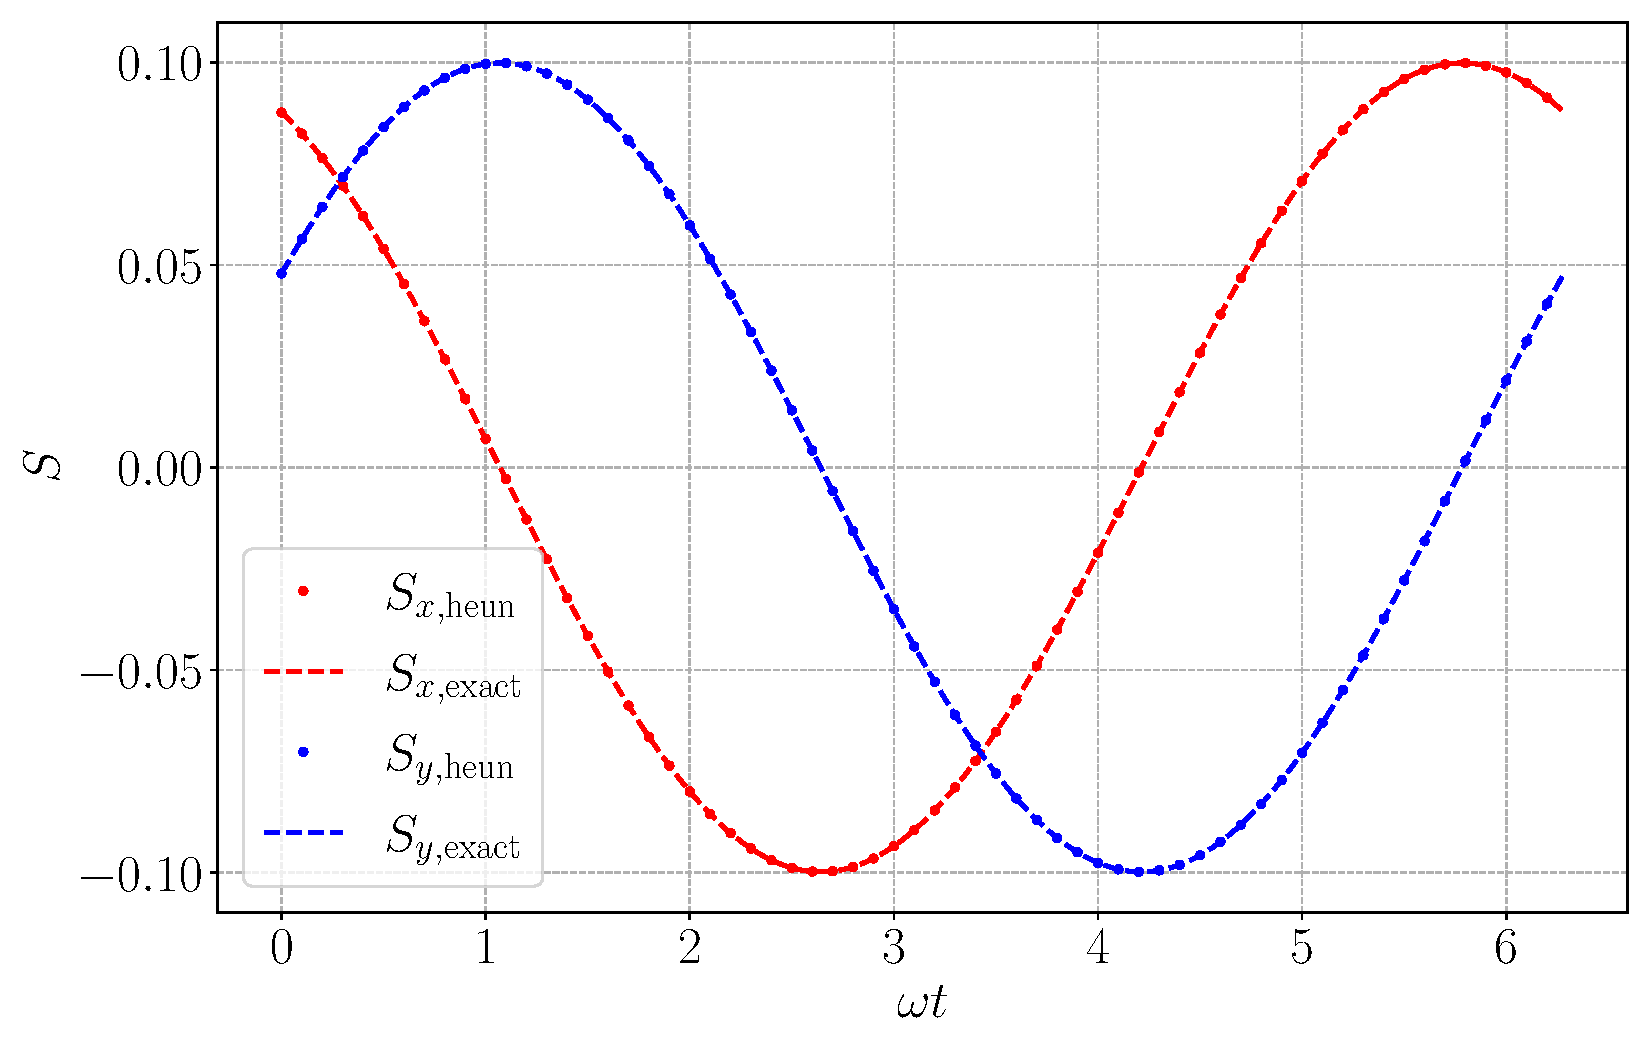
\includegraphics[width=\columnwidth]{../fig/comparison.pdf}
	\caption{The plot shows the exact solution given in \eqref{eq:exact_1} and \eqref{eq:exact_2} compared with the numerical solution sampled at every tenth step to be able to distinguish the paths.}
	\label{fig:comp}
\end{figure} 

It is perhaps more enlightening to consider the pointwise difference of the exact and numerical solution. This is shown in figure \ref{fig:comp_diff}. The figure shows that the deviations locally oscillate, but globally, of course, the absolute deviation increases.

\begin{figure}[htb]
	\centering
	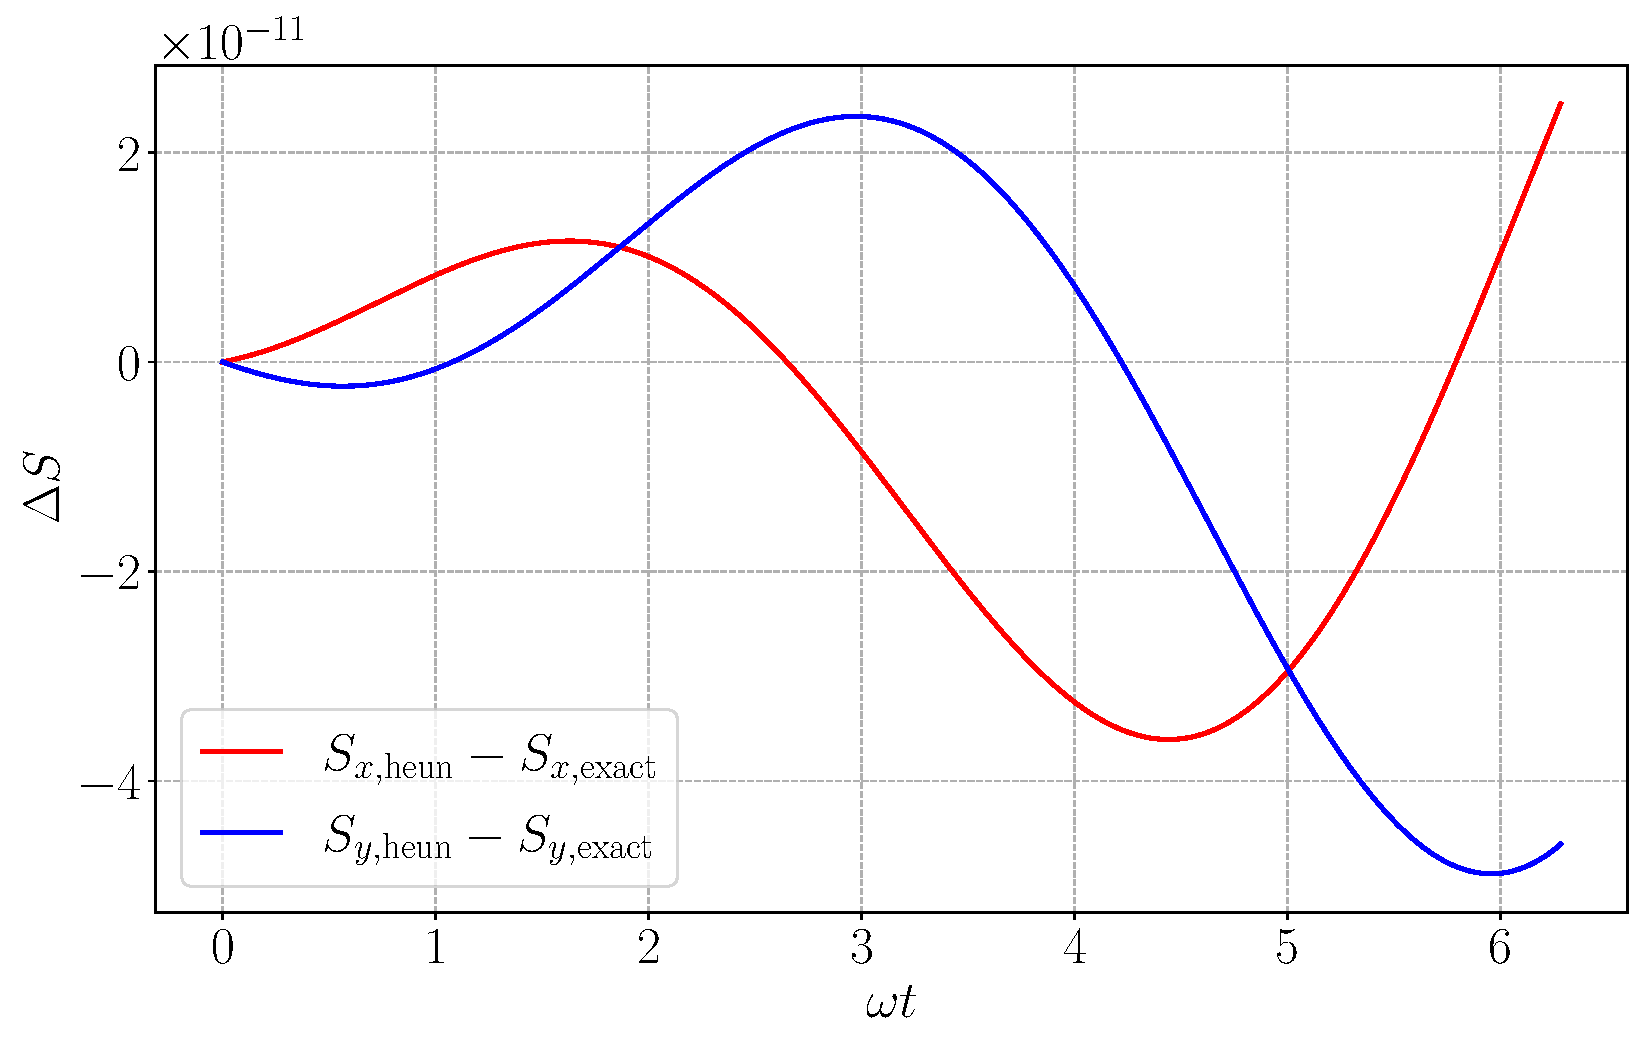
\includegraphics[width=\columnwidth]{../fig/comparison_diff.pdf}
	\caption{The plot shows the difference between the exact solutions given in \eqref{eq:exact_1} and \eqref{eq:exact_2}, and the numerical solutions over one period.}
	\label{fig:comp_diff}
\end{figure} 
\section{The spin chain}

\subsection{Ground states}

In this section we initialise $10$ spins in random directions and simulate the time evolution for $J <0$ and $J>0$. The plots of the $z$-component of each of the spins over time is shown in figure \ref{fig:ferro} and \ref{fig:antiferro}. What is evident from these plots is that a positive coupling constant $J$ tends to make the spins align with their neighbours, while the negative constant tends to make them oppose them. This is a fact that is readily seen from inspecting the hamiltonian in \eqref{eq:hamiltionian}, since a positive $J$ makes the maximum of $\sum_{j,k} \mathbf{S}_j \cdot \mathbf{S}_k$ most energetically favourable, while a negative one makes its minimum most favourable. These two cases correspond to a ferromagnetic and anti-ferromagnetic system respectively.

The reason for this being apparent when only plotting the $S_z$-component is the non-zero anisotropy-constant $d_z$. As seen from the hamiltonian, setting this positive will favour spins in the $z$-direction. This is also the reason that approximately half of the spins in the case of $J<0$ being directed along $\mathbf{e}_z$ while the others are directed along $-\mathbf{e}_z$.

\begin{figure}[htb]
	\centering
	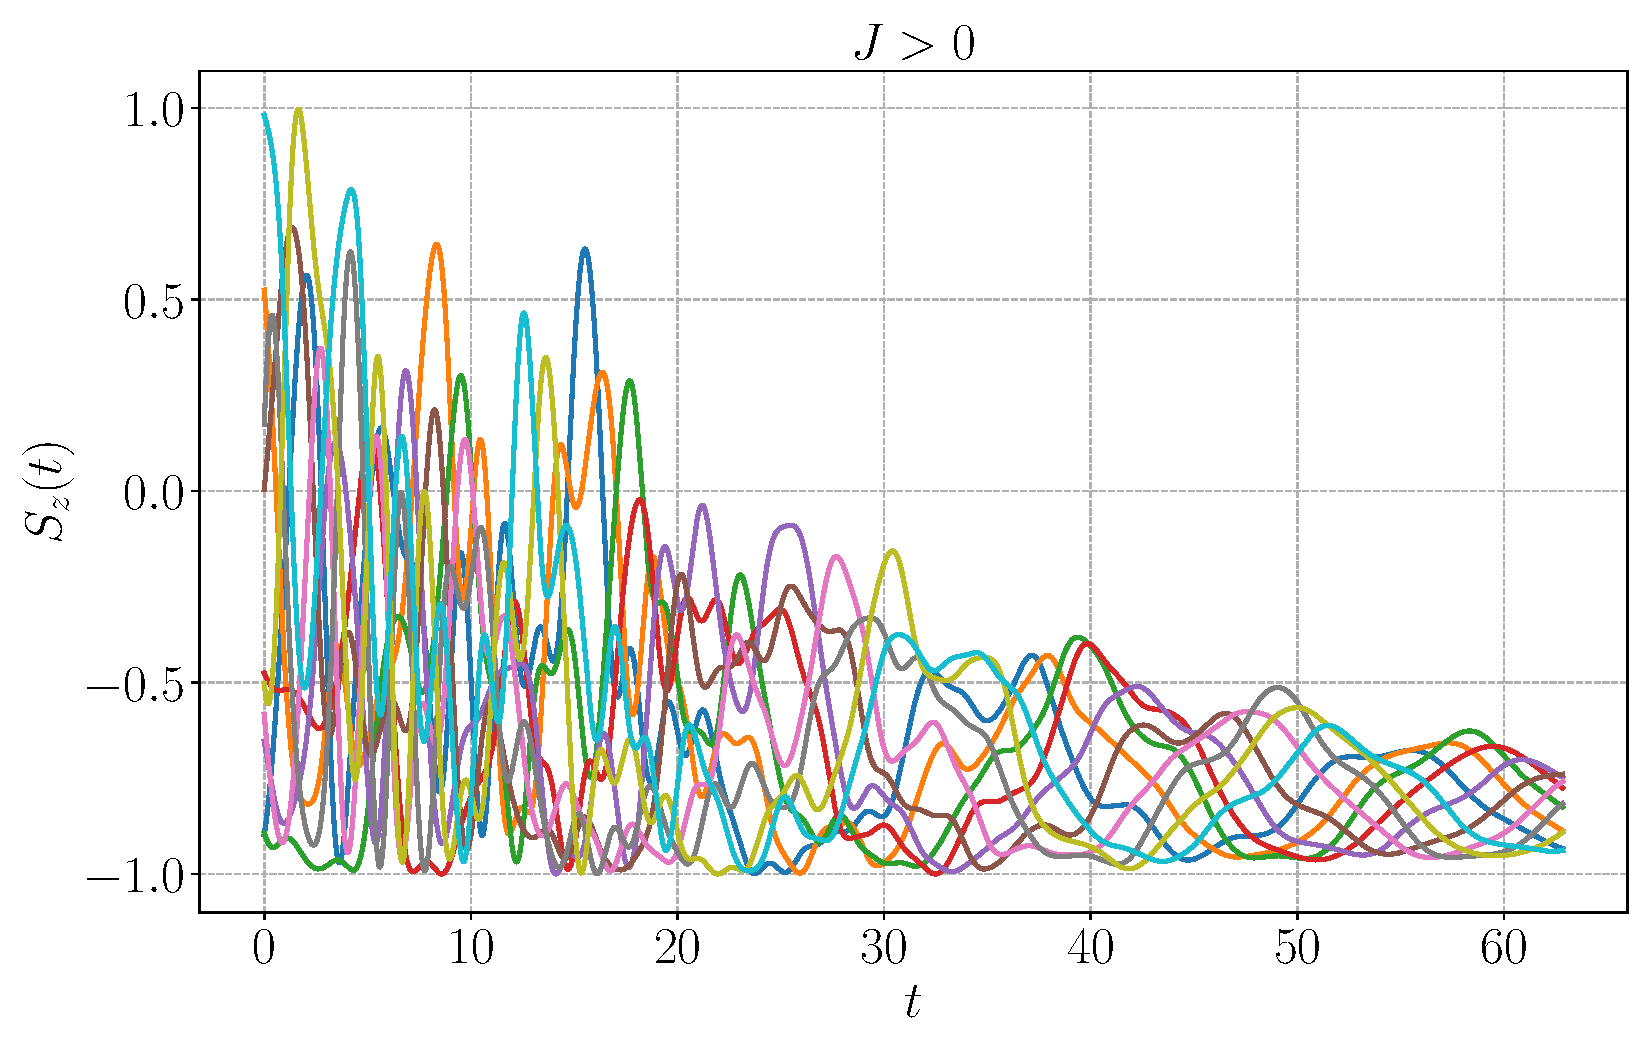
\includegraphics[width=\columnwidth]{../fig/gs_ferro.pdf}
	\caption{The figure shows the plot of the $z$-component of the spin of $10$ spins in a system of positive coupling constant $J > 0$.}
	\label{fig:ferro}
\end{figure}

\begin{figure}[htb]
	\centering
	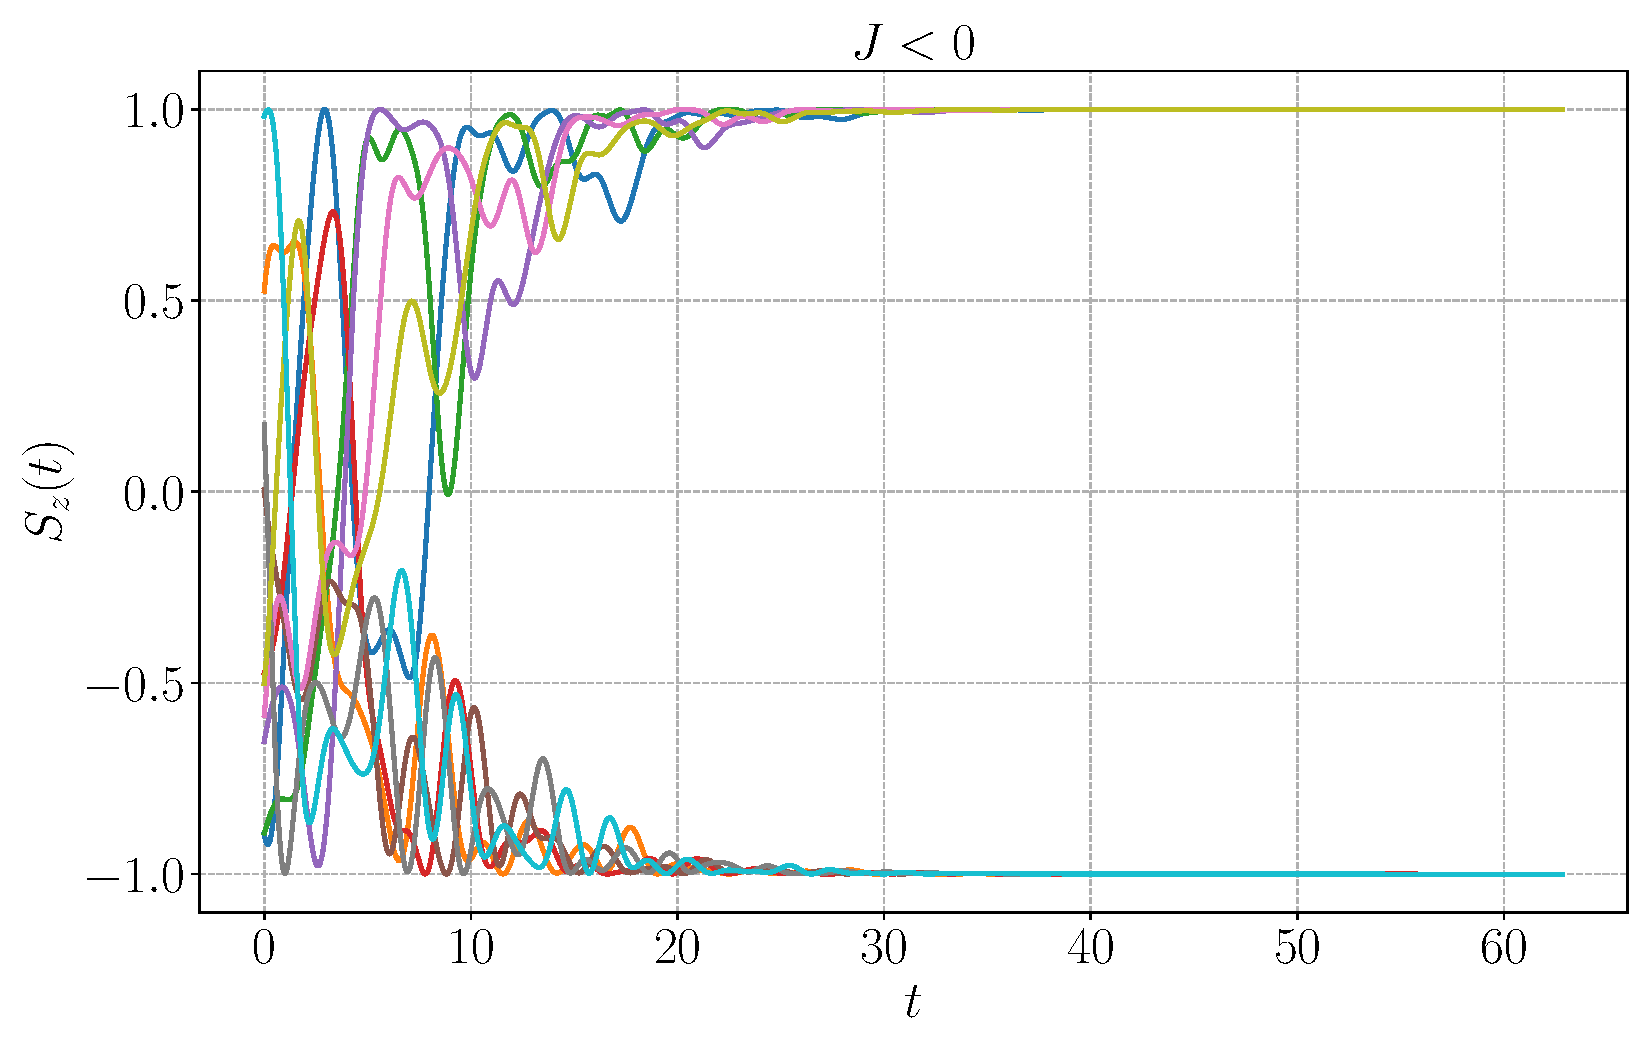
\includegraphics[width=\columnwidth]{../fig/gs_antiferro.pdf}
	\caption{The figure shows the plot of the $z$-component of the spin of $10$ spins in a system of negative coupling constant $J < 0$.}
	\label{fig:antiferro}
\end{figure}

\subsection{The magnon}

\subsubsection{Uncoupled system}

We initialise the system of $10$ spins with random orientations in space and set $J = 0$, $d_z = 1$, $\alpha = 0$ to demonstrate that all the spins precess in time. The trajectories of the $x$ and $y$ components of the spins is plotted in figure \ref{fig:precessionsxy}

\begin{figure}[htb]
	\centering
	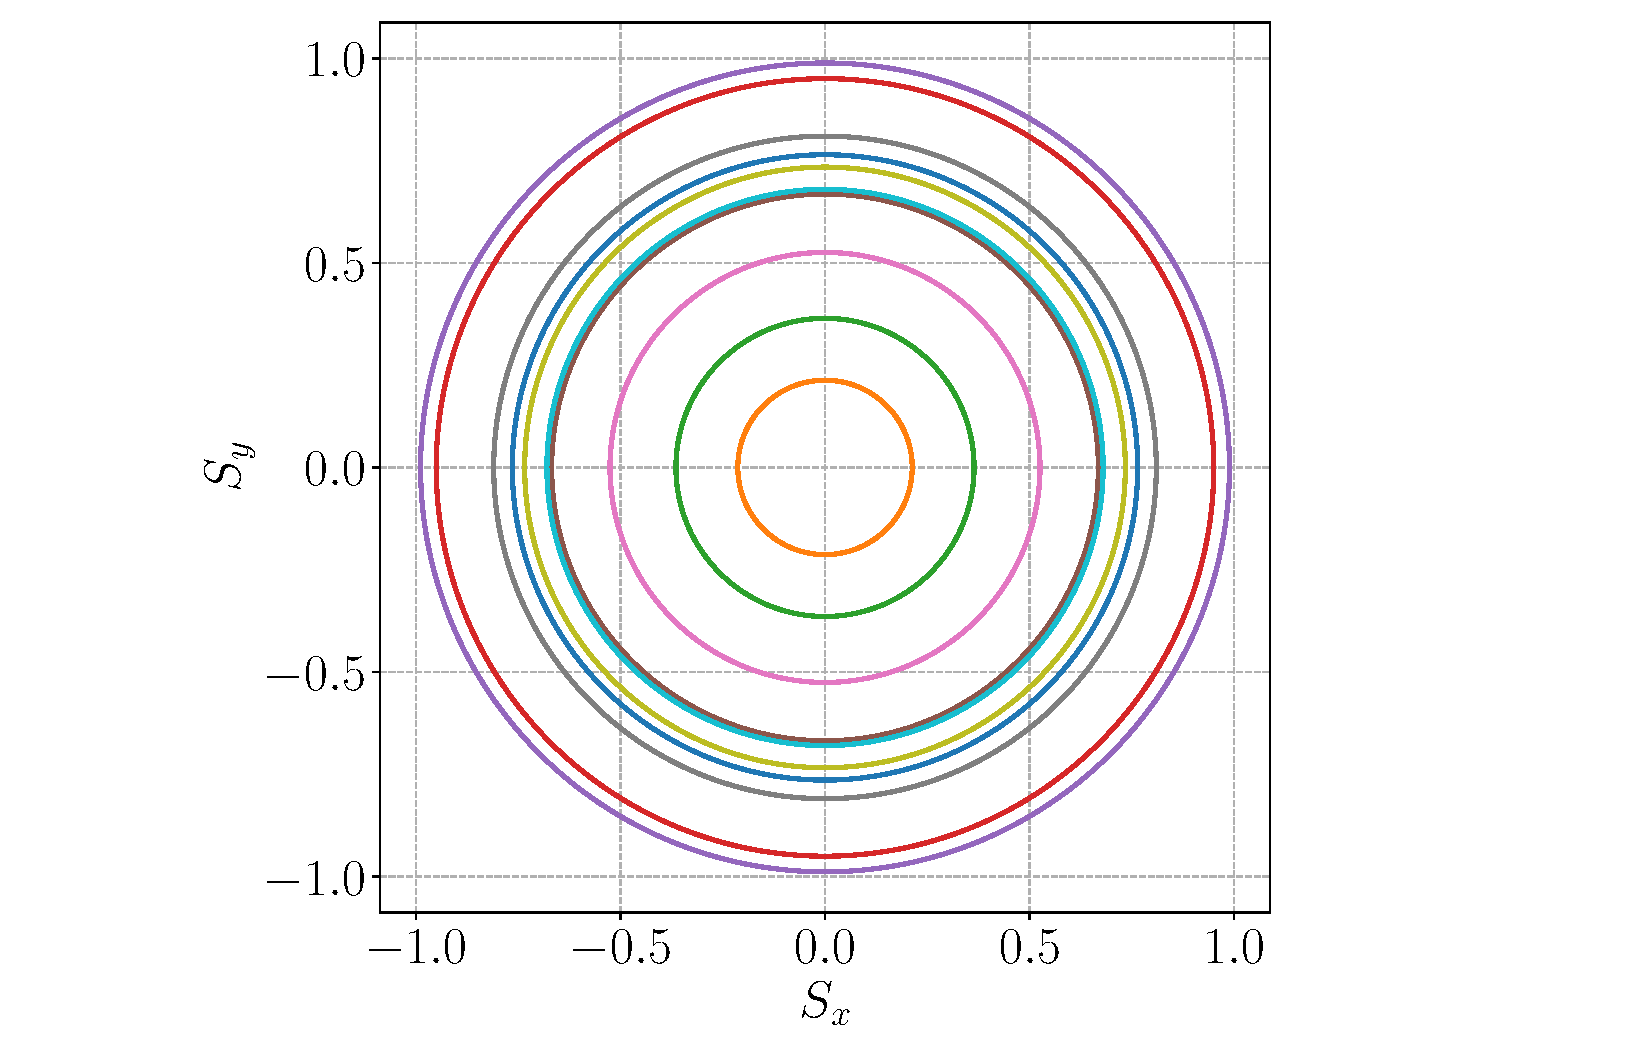
\includegraphics[width=0.8\columnwidth]{../fig/precession_xy.pdf}
	\caption{Trajectories of the $x$ and $y$ components of the $10$ randomly initialised spins.}
	\label{fig:precessionsxy}
\end{figure}

Next, we initialise all the spins along the $z$ direction except for one of them which we tilt slightly. Since there is no coupling between the spins, the precession of the first spin will not affect the others. Furthermore, when $\mathbf{S} = S\mathbf{e}_z$, the right hand side of the LLG \eqref{eq:llg} will be zero since the effective field is $\parallel \mathbf{e}_z$. As expected, this is also what is observed when simulating the system. This is shown in figure \ref{fig:precessions}.

\begin{figure}[htb]
	\centering
	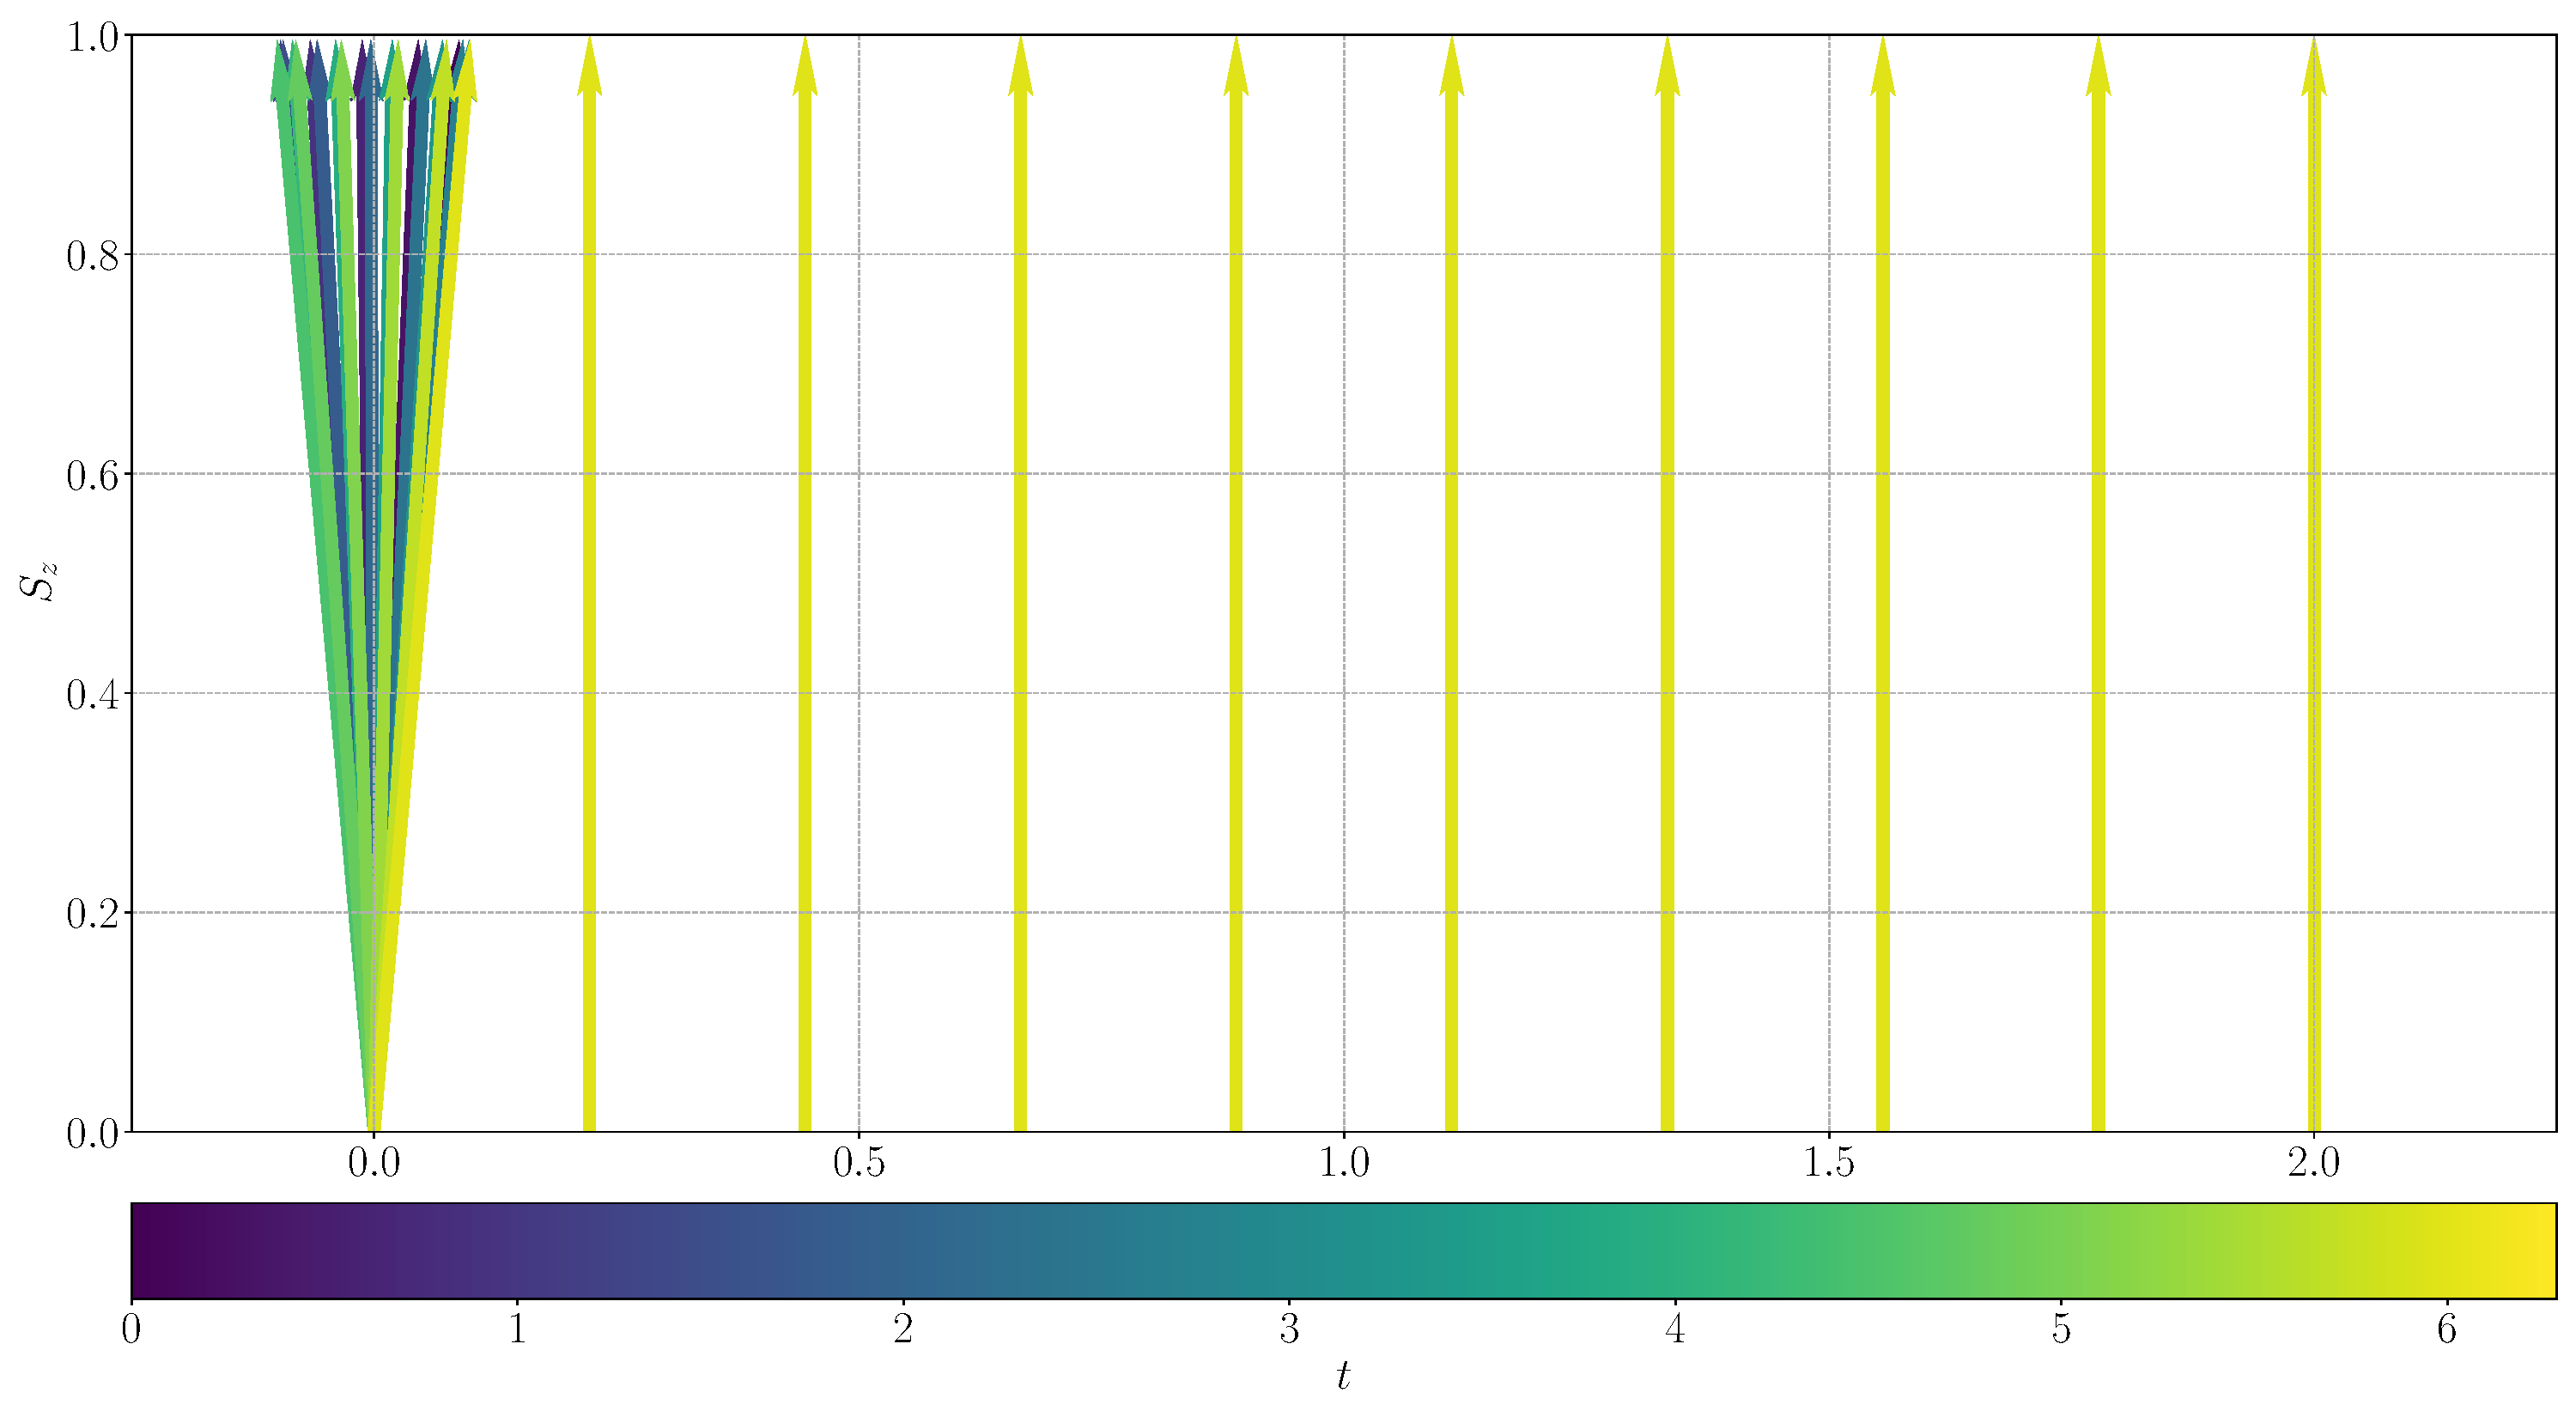
\includegraphics[width=\columnwidth]{../fig/10_precessions.pdf}
	\caption{The figure shows uncoupled oscillations of the spin chain.}
	\label{fig:precessions}
\end{figure}

\subsubsection{Coupled system}

If we repeat the procedure used in the previous section except that we couple the spins with $J > 0$, we will observe that all the spins will start to precess, even if they are initialised along the $z$-axis. This is shown in figure \ref{fig:coupled_precessions}. Since the time evolution is hard to catch on a $2\mathrm{d}$ plot I have made a video showing the same as figure \ref{fig:coupled_precessions} \href{https://folk.ntnu.no/sondrdl/spinwaves/coupled.mp4}{here}. What is apparent here is that the neighbouring spins couple to each other. Since we are dealing with a finite system, I have chosen to use periodic boundary conditions, so that the first spin affects the last one and vice versa. Implementing this in python requires no effort at all as we can access the left hand neighbour of spin \texttt{i} with \texttt{i-1} regardless of the value of \texttt{i}, and the right hand neighbour with \texttt{(i-1)\%n} where \texttt{n} is the number of spins. This looks a bit artificial in the video, but it corresponds physically to arranging the linear chain in a circle. Another choice of boundary conditions is to simply say that the first and last spin only has \textit{one} neighbour. 

\begin{figure}[htb]
	\centering
	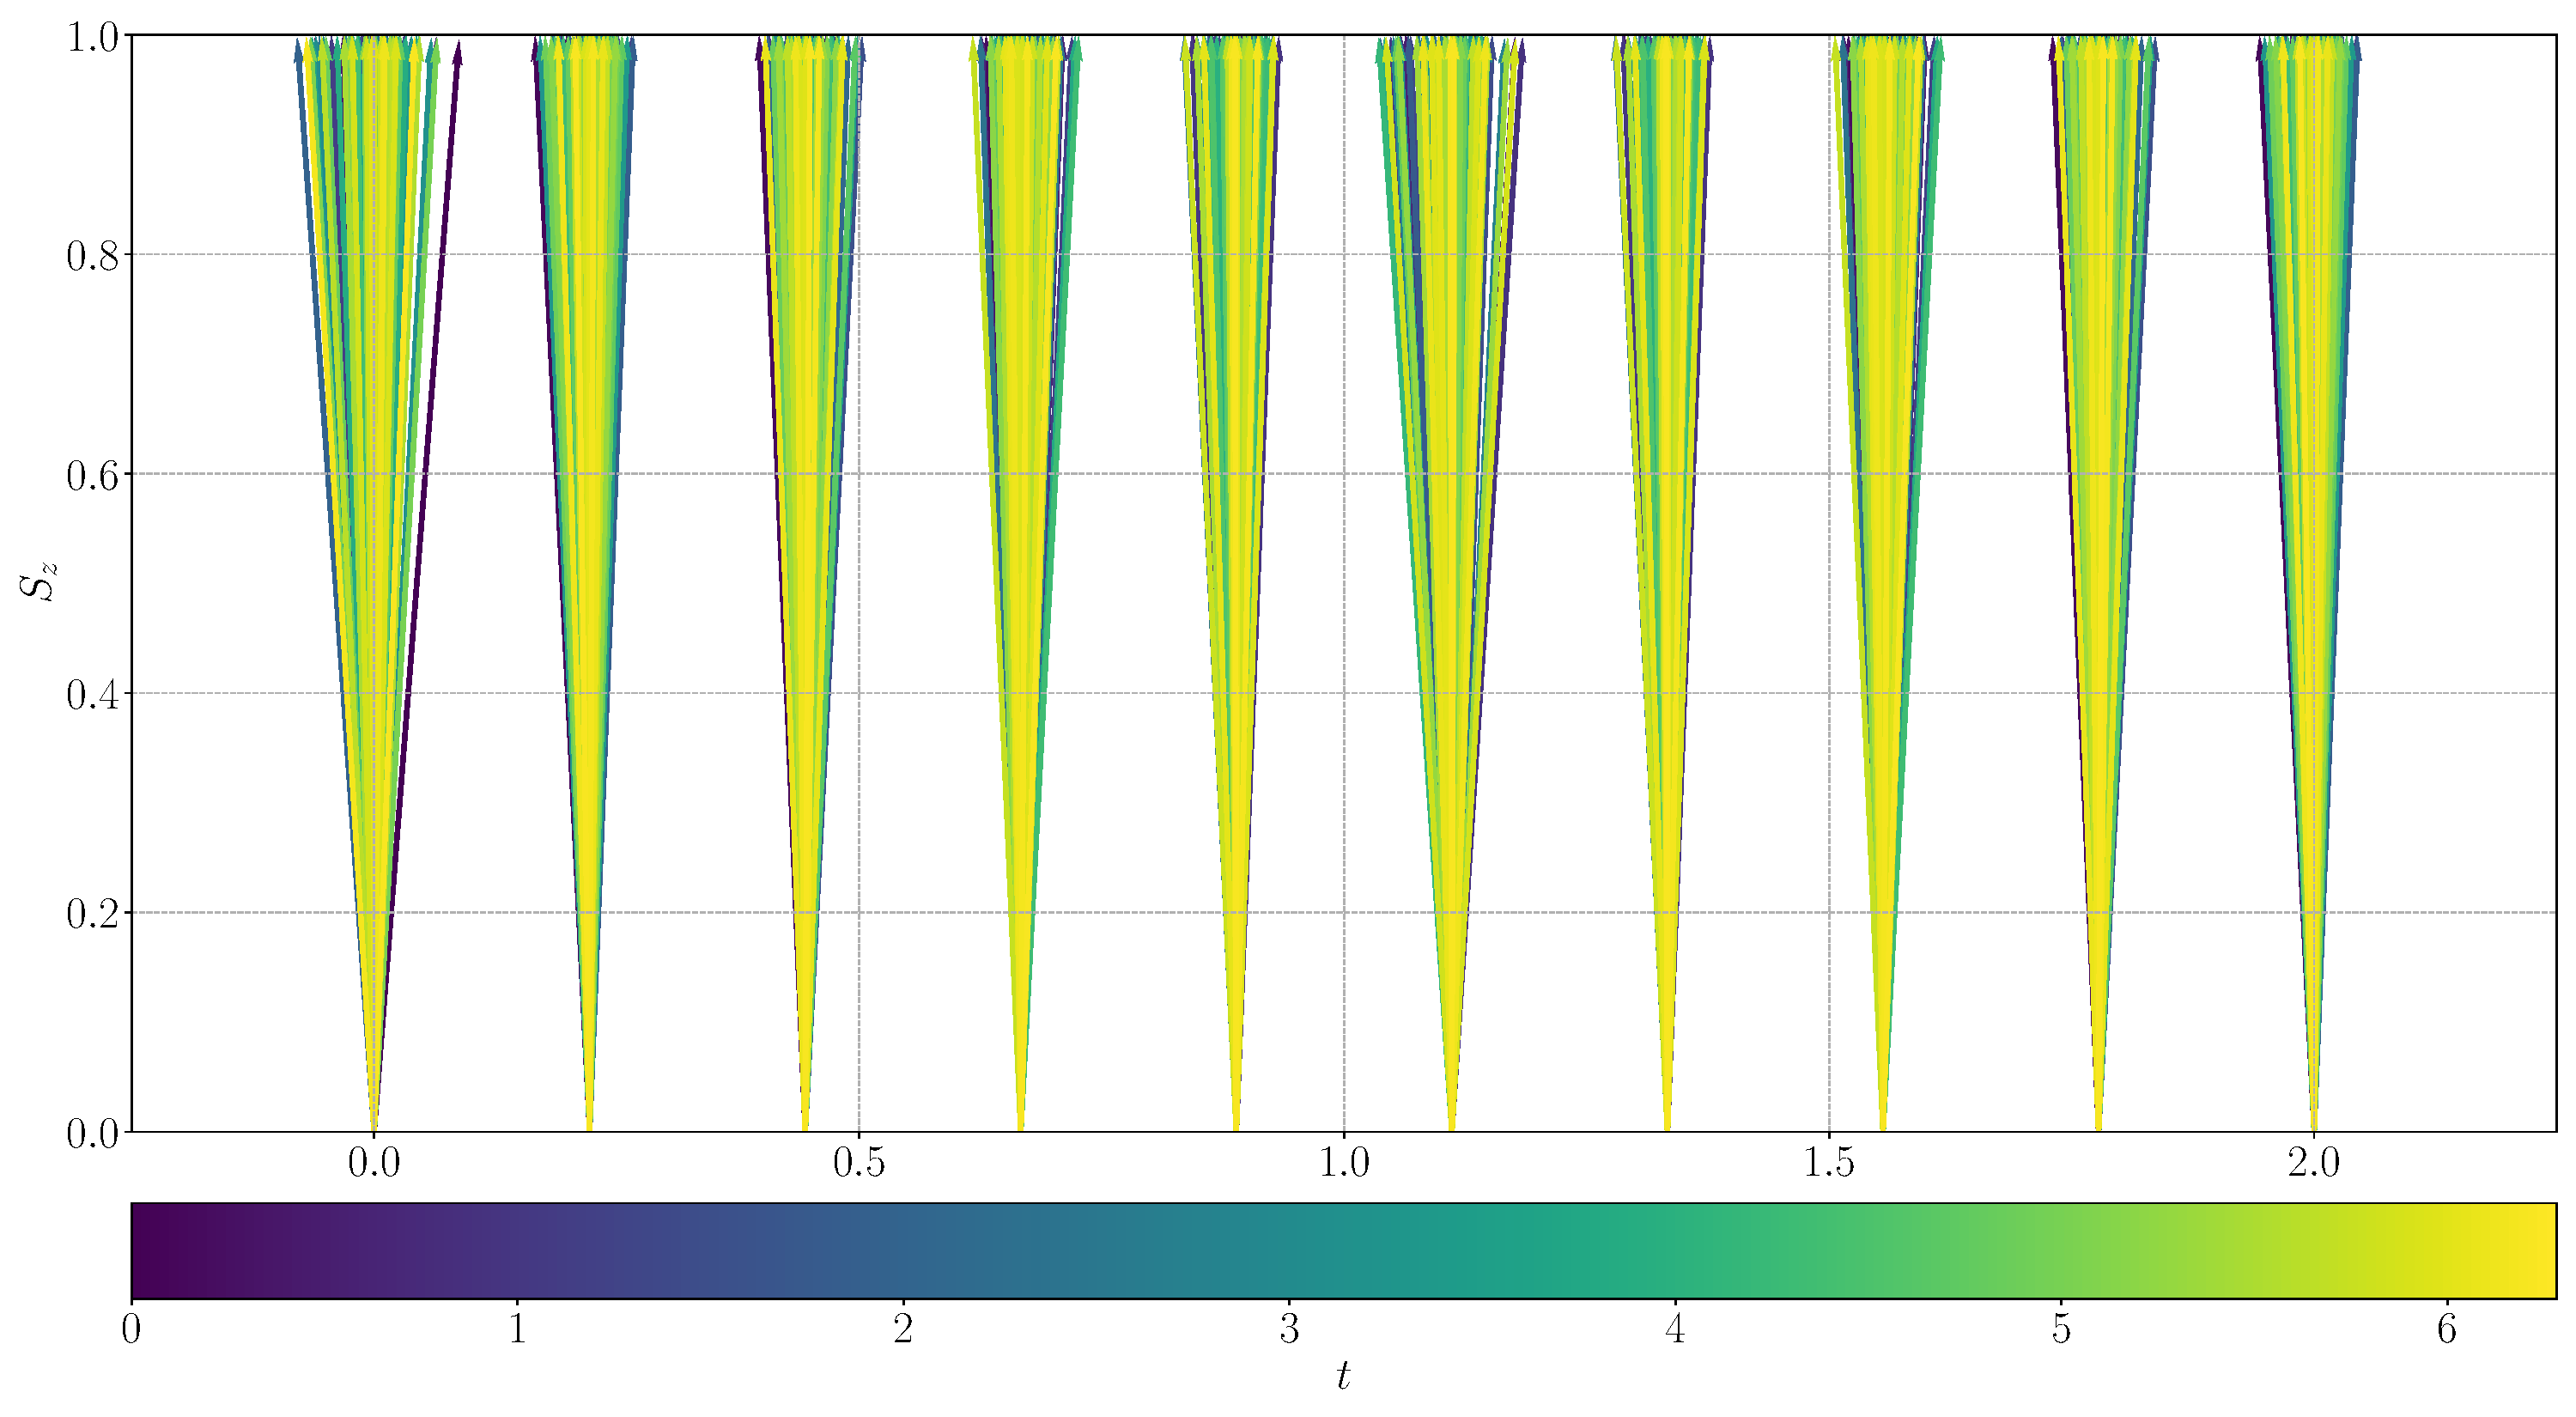
\includegraphics[width=\columnwidth]{../fig/10_precessions_coupled.pdf}
	\caption{The figure shows coupled oscillations of the spins. A video displaying the same data set can be found \href{https://folk.ntnu.no/sondrdl/spinwaves/coupled.mp4}{here}.}
	\label{fig:coupled_precessions}
\end{figure}

If we are to simulate an infinite system we obviously cannot use a discrete model. However, the simulations above suggests that in the limit of \textit{many} spins we can describe the chain as a continuous wave. Then we would have to associate to every index $j$ a position in space 
$$
	\mathbf{S}_j(t) \to \mathbf{S}(\mathbf{x},t) \quad ; \quad j \to \mathbf{x},
$$
where $\mathbf{x}$ is the position of spin $j$.
If we approximate the directional derivatives along a lattice vector $\mathbf{a}$ by the finite differences 
$$
	 \|\mathbf{a}\|^2  \nabla^2 \mathbf{S}(\mathbf{x},t) \approx \|\mathbf{a}\|^2 \frac{\mathbf{S}(\mathbf{x} - \mathbf{a},t) - 2 \mathbf{S}(\mathbf{x},t) + \mathbf{S}(\mathbf{x} + \mathbf{a},t) }{ \| \mathbf{a} \|^2}
$$
and 
$$
	\mathbf{a} \cdot \boldsymbol{\nabla} \mathbf{S}(\mathbf{x},t) \approx \|\mathbf{a}\| \frac{\mathbf{S}(\mathbf{x}+\mathbf{a},t) - \mathbf{S}(\mathbf{x}-\mathbf{a},t)}{2\|\mathbf{a}\|},
$$
we see that 
$$
	\mathbf{S}_{j-1}(t) + \mathbf{S}_{j+1}(t) \to \mathbf{S}(\mathbf{x},t) + \mathbf{a} \cdot \boldsymbol{\nabla} \mathbf{S}(\mathbf{x},t) + \frac{\| \mathbf{a} \|^2}{2} \nabla^2 \mathbf{S}(\mathbf{x},t) + \mathcal{O}(\|\mathbf{a}\|^2).
$$
Hence, in the limit of small lattice spacings $\|\mathbf{a}\| \to 0$ it should be possible to recast the LLG equation in a continuous form, as a PDE rather than an ode. A self contained discussion of this can be found in \cite{Lakshmanan2011}.

\newpage
\part{Conclusion}
We have simulated the time evolution of various spin chains governed by different Hamiltonians. When there is non-zero coupling between the spins the local excitations propagate along the spins like a wave. This demonstrates the emergence of \textit{magnons}, which - much like phonons - are quantised waves, which only resemble real wave behaviour in the limit of infinitely many spins.

\bibliographystyle{unsrt}
\bibliography{references}

\end{document}